\paragraph{Sơ đồ tuần tự luồng Lấy thông tin Cài đặt}

Luồng nghiệp vụ này mô tả
quy trình Web Frontend
truy vấn danh sách cài đặt cá nhân của người dùng
từ Setting Service (Neon API) thông qua API Gateway.

\begin{figure}[H]
\centering
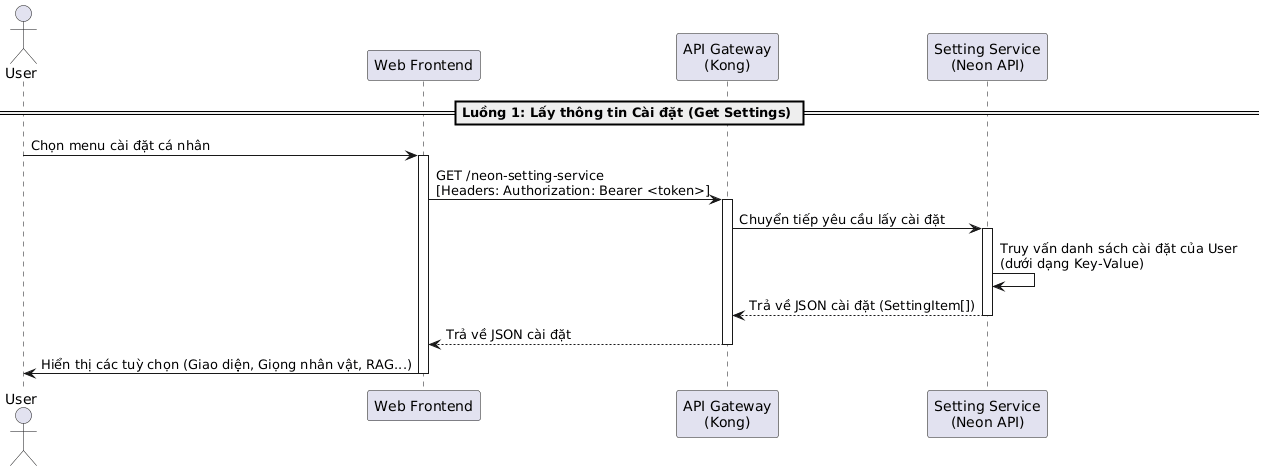
\includegraphics[scale = 0.2]{contents/Sequence/UML-Sequence-UserGetSettings.png}
\caption{Sơ đồ tuần tự luồng Lấy thông tin Cài đặt}
\end{figure}

\subparagraph{Các thành phần tham gia}

\begin{table}[H]
\centering
\renewcommand{\arraystretch}{1.3}

\begin{tabular}{|l|l|p{5cm}|}
\hline
\textbf{Thành phần} & \textbf{Phân loại} & \textbf{Vai trò trong hệ thống} \\ \hline
User & Actor & Người dùng thực hiện xem cấu hình cài đặt. \\ \hline
Web Frontend & Component & Giao diện web Next.js. \\ \hline %%%% Component & Giao diện Next.js hiển thị trạng thái các tùy chọn cấu hình. \\ \hline
API Gateway (Kong) & Component & Cổng API chuyển tiếp các yêu cầu API. \\ \hline %%%% Component & Định tuyến yêu cầu lấy cấu hình cài đặt. \\ \hline
Setting Service (Neon API) & Microservice & Dịch vụ quản lý và truy vấn các cấu hình cài đặt của người dùng. \\ \hline
\end{tabular}
\caption{Các thành phần tham gia luồng Lấy thông tin Cài đặt}
\end{table}

\subparagraph{Mô tả tổng quan}

\begin{itemize}
\item \textbf{Yêu cầu lấy cài đặt:} Người dùng truy cập vào trang cấu hình cài đặt. Giao diện gửi yêu cầu lấy thông tin cài đặt qua cổng API tới dịch vụ cấu hình cài đặt kèm theo mã phiên đăng nhập.
\item \textbf{Phản hồi cấu hình:} Dịch vụ cấu hình cài đặt truy vấn danh sách các cài đặt cá nhân của người dùng dưới dạng các cặp khóa và giá trị từ cơ sở dữ liệu cài đặt và phản hồi về giao diện để hiển thị cho người dùng.
\end{itemize}
